\section{Sprint 4: Gestión de Usuarios}
    \begin{description}
        \item \textbf{Duración}: 15 días.
        \item \textbf{Inicio del sprint }: 11 de marzo de 2022.
        \item \textbf{Cierre del sprint }: 25 de marzo de 2022.
    \end{description}

    \subsection{Planeación}

    Esta iteración tuvo como propósito implementar un mecanismo que permita a los usuarios del sistema autenticarse y/o crear cuentas
    para acceder al mismo, las actividades realizadas fueron:
    \begin{enumerate}
        \item Se diseñó e implementó las interfaces de usuario para la gestión de cuentas y accesos.
        \item Se especificaron los requerimientos mediante casos de uso con sus respectivas interfaces de usuario.
        \item Se elaboró el a de casos de uso para este sprint.
        \item Se elaboró la maquina de estados de un reclutador.
    \end{enumerate} 

    Los requerimientos funcionales de este sprint se muestran en la siguiente tabla.
    \begin{requerimientos}{funcionales}
        \RFitem{RF-GRL-01}{Iniciar sesión}{El sistema debe proporcionar un mecanismo que permita al actor acceder al sistema mediante un correo y una contraseña.}
        \RFitem{RF-GRL-02}{Crear cuenta}{El sistema debe proporcionar un mecanismo que permita al actor registrarse como nuevo usuario en el sistema.}
        \RFitem{RF-USR-04}{Consultar perfil}{El sistema debe permitir al actor acceder a su perfil para consultar la información registrada.}
        \RFitem{RF-USR-05}{Editar perfil}{El sistema debe permitir al actor modificar la información registrada en su perfil, como nombre, apellidos, información de contacto y si el usuario es un candidato, debe de permitir modificar su información académica y datos de habilidades y conocimientos del mismo.}
        \RFitem{RF-EM-24}{Enviar solicitud para acceder al sistema}{El sistema debe proporcionar un mecanismo para que al representante de una empresa pueda enviar una solicitud o pre-registro de poder acceder y publicar vacantes.}
    \end{requerimientos}

    Los casos de uso que se describieron en este sprint pertenecen al \textbf{Módulo General (GRL)} el cual tiene como objetivo 
    permitir el acceso al sistema para todos los actores y al \textbf{Módulo de Usuarios (USR)} la configuración del perfil de usuario dentro del sistema.

    En la figura \ref{dcu:MUSR} se puede ver el diagrama de casos de uso del \textbf{Módulo de Usuarios (USR)}:
    \begin{itemize}
        \item Los casos de uso \IUazul{} , son aquellos que se van implementar en este sprint.
        \item Los casos de uso \IUblanco{}, se tienen planeados para sprints posteriores.
    \end{itemize} 

   

    \begin{figure}[H]
        \begin{center}
            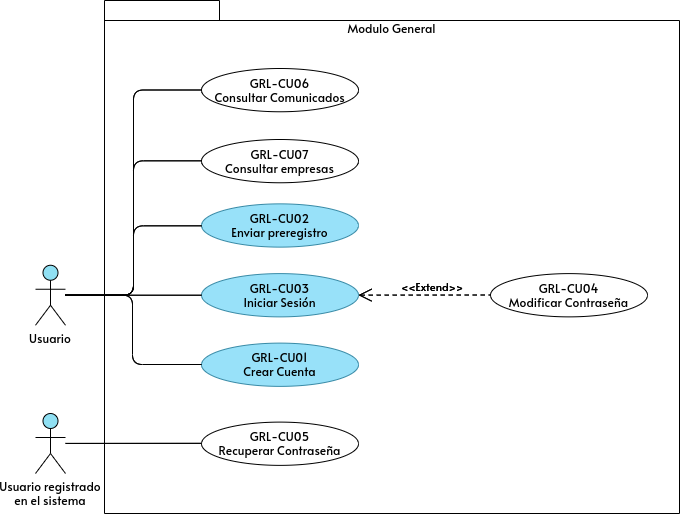
\includegraphics[width=.7\textwidth]{sprints/imagenes/CUGRL.png}
        \end{center}
        \caption{Diagrama de casos de uso del \textit{Módulo General}.}
        \label{dcu:MUSR}
    \end{figure}

    A continuación se listan los casos de uso de este sprint:
    \begin{itemize}
        \item \refElem{GRL-CU01}
        \item \refElem{GRL-CU02}
        \item \refElem{GRL-CU03}
        %\item \refElem{USR-CU02-2}
    \end{itemize} 


    \subsection{Ejecución}
        El \textit{Módulo General} fue el primero en desarrollarse ya que permite conocer el tipo de usuario
        que está ingresando al sistema.\\ 
        
        Se implementó JSON Web Token basado en algoritmo HASH 256 para la creación de tokens al iniciar sesión, cuyo objetivo es 
        autentificar la identidad del usuario.y sus datos ingresados. Fue necesario utilizar la bibliotea \textit{JSON web token} 
        la cual es deribada de la bibliotea \textit{djangorestframework}
        %En la figura  se muestra un diagrama de flujo en el que se describe el uso del Web Token en el sistema. 

        Al utilizar Django, se crea por defecto una tabla generica llamada \textit{users} la cual nosotros seleccionamos
        la version por defecto miníma, de esta forma pudimos utilizar las funciones del JSON Web Token y a su vez la modificamos 
        de tal forma que pudieramos cubrir los requerimientos de este sprit.
        %\clearpage
        En la figura \ref{tbdb:users} se muestra la tabla \textit{users} tal como utiliza en el sistema. 
        \begin{figure}[H]
            \begin{center}
                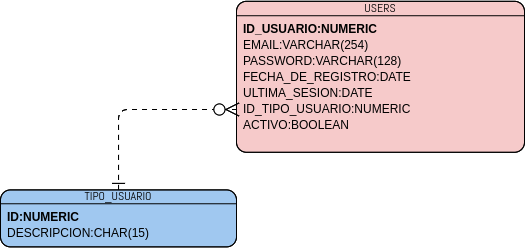
\includegraphics[width=.7\textwidth]{sprints/imagenes/sp1mdd.png}
            \end{center}
            
            \caption{Tabla \textit{users}.}
            \label{tbdb:users}
        \end{figure}
    
       %En la figura  se muestra el funcionamiento del  Web Token ya implentado en el sistema.

       \subsection{Revisión y retroalimentación}
       Antes de liberar los casos de uso programados de este sprit, fue validado su funcionamiento:
        \begin{enumerate}
            \item Se utilizo el sistema siguiendo cada caso de uso al pie de la letra segun su descripción y trayectorias. 
            \item Se hicieron las pruebas unitarias por cada campo, validando que el tipo de dato ingresado fuera correcto y en caso de no 
            hacerlo mostrara el mensaje correcto según lo indicado en el caso de uso.

            \item Se hicieron las pruebas unitarias por cada botón, validando que redireccionara a la interfaz correcta y/o mostrara el mensaje
            correcto egún lo indicado en el caso de uso.
        \end{enumerate} 
       Para este sprint en específico se hicieron pruebas para el componente JSON Web Token a través de este 
       framework se puede autentificar el acceso del usuario al sistema, al iniciar sesión con un usuario 
       registrado en el sistema se comprueba que existe un usuario con el ``username'' enviado y de existir 
       se compará la contraseña enviada con la almacenada para ese usuario, aplicando el mismo algoritmo que
     se usa para encriptar las contraseñas, si la información coincide se devuelve un objeto JSON con el token de autentificación, el token de refresh e información del usuario al FrontEnd por medio de la API creada.

    


